\section{Specification Analysis}
\label{sec:spec-analysis}

\subsection{Thematic Structure}
The distributions show which obligation types dominate each extracted corpus, while clause mappings establish their normative force and schema enforcement. SPDX is profile-driven and graph-oriented: 57\% of its extracted rows are class-specific, mostly constraining structure rather than content. In CycloneDX (Table~\ref{tab:cdx_theme_distribution}), provenance, identity, and trust leads with 585 rows (33.9\%), followed by specialized security models with 397 (23.0\%); dependency and downstream-use semantics account for 32 (1.9\%). The mapped clauses show where a valid artifact may leave provenance, filtered dependencies, or empty graph entries unexplained.

\begin{tcolorbox}[colback=gray!4!white, colframe=black!80, boxrule=0.5pt, arc=5pt, left=2pt, right=2pt, top=1pt, bottom=1pt]
\textbf{Key Takeaway:} The extracted corpora emphasize structural and class-specific rules. Dependency coverage and explicit meanings for missing data receive less baseline guidance, creating the interface boundaries analyzed below.
\end{tcolorbox}

\subsection{CISA: Mandatory Process, Softer Data Quality}
\begin{figure}[t]
    \centering
    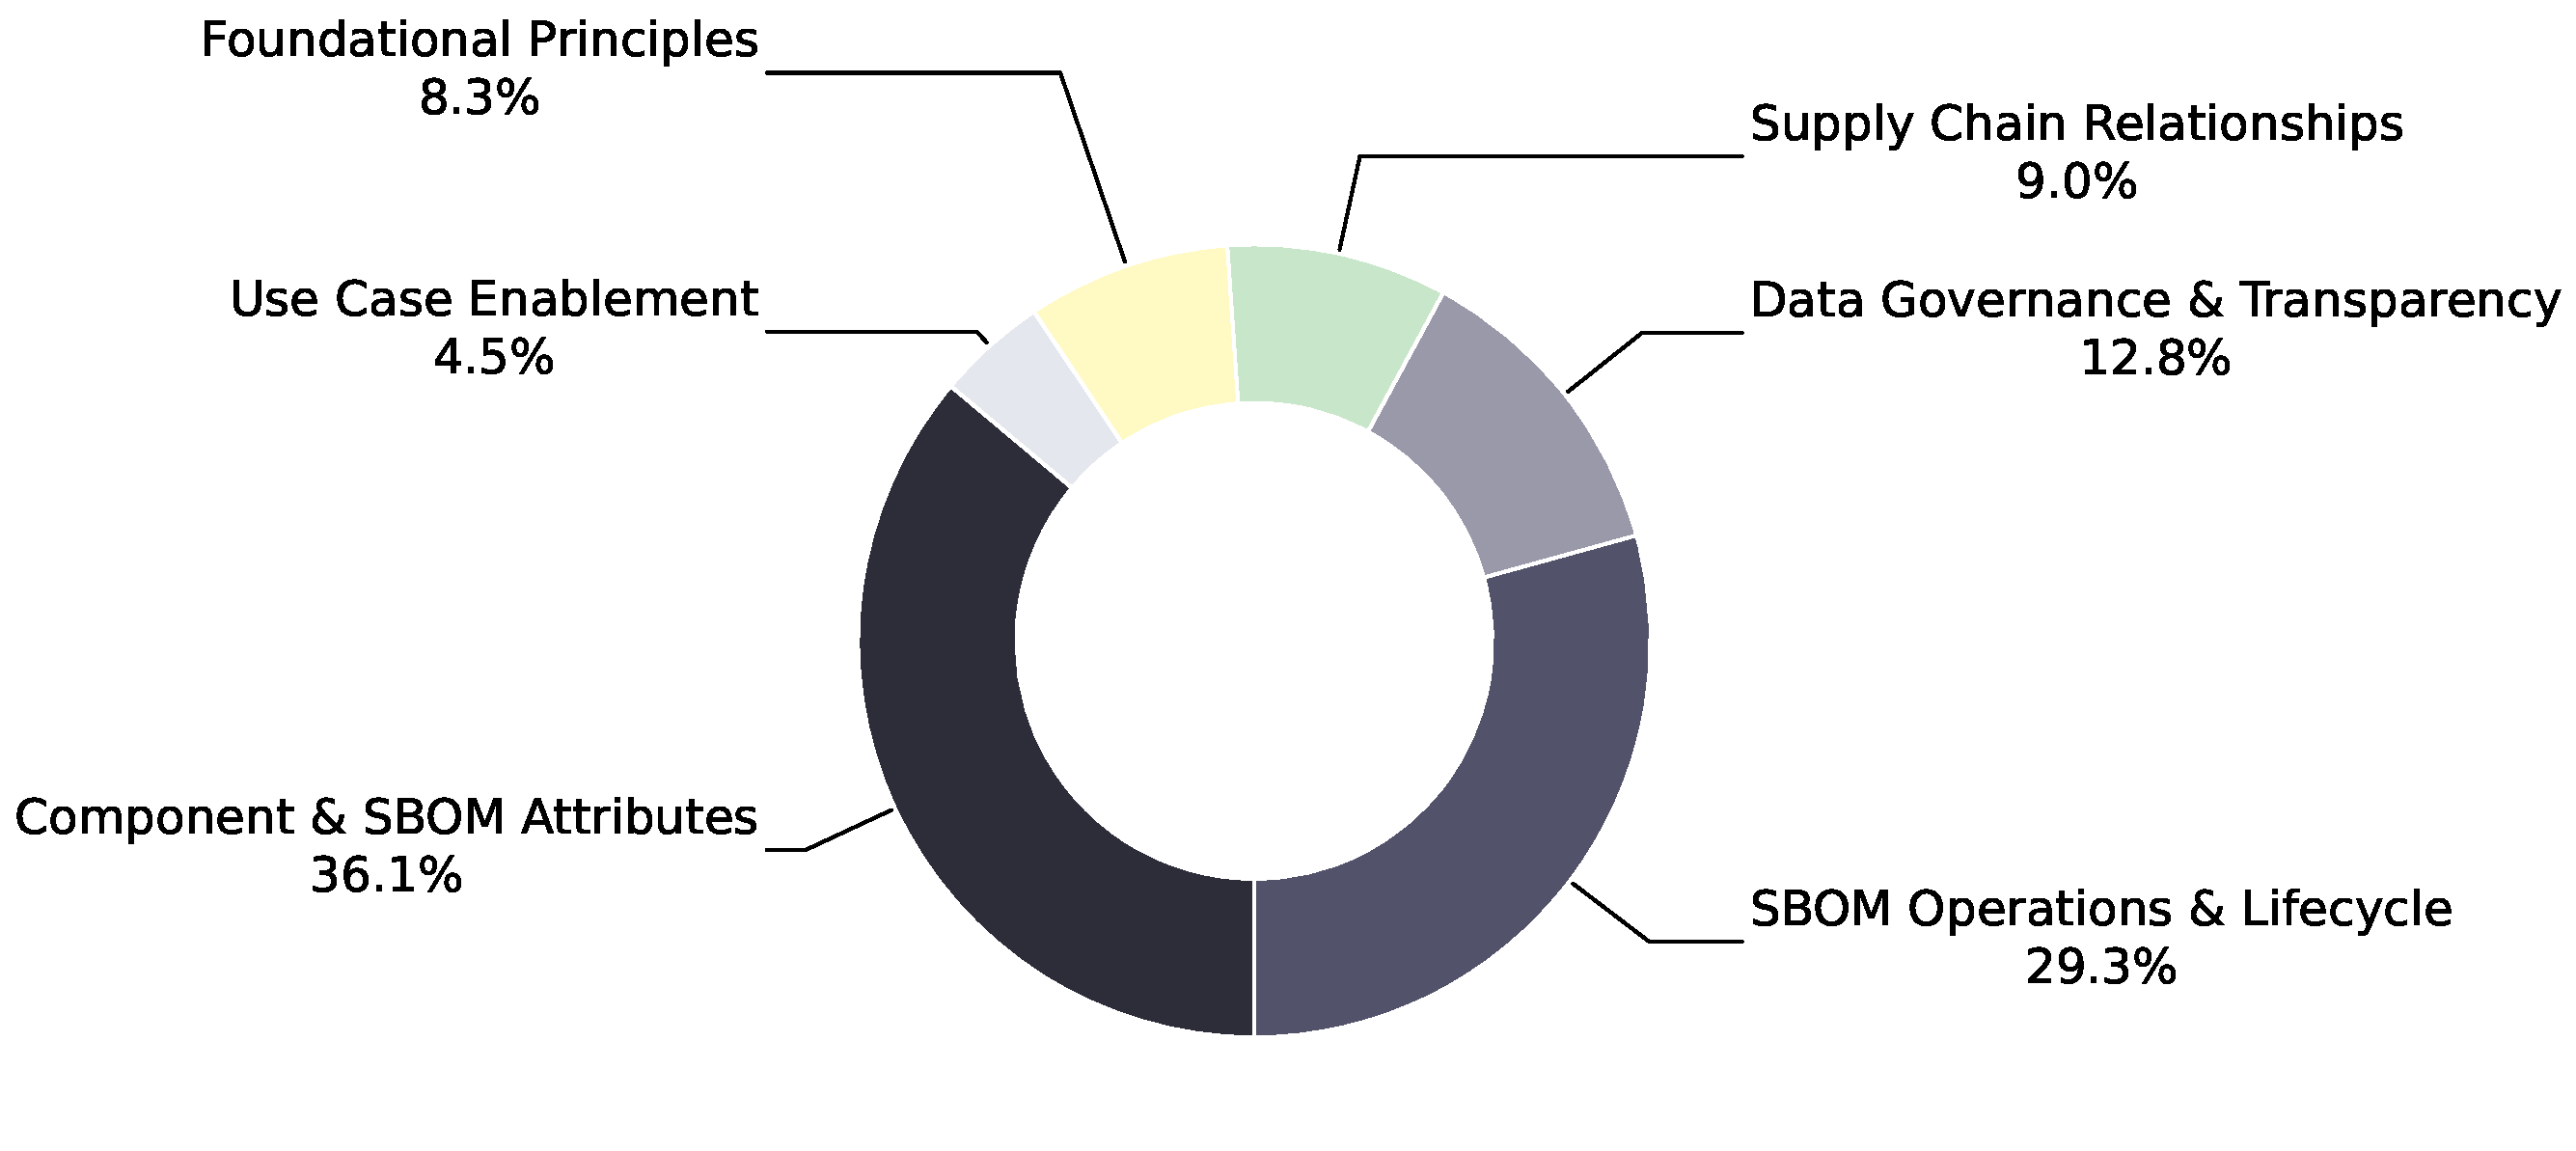
\includegraphics[width=\columnwidth]{figures/cisa_theme_pie.pdf}
    \vspace{-2.5em}
    \caption{CISA themes within the 133-row extracted corpus.}
    \Description{Pie chart of the 133 extracted CISA rows. Component and SBOM Attributes is the largest theme at 36.1 percent, followed by SBOM Operations and Lifecycle at 29.3 percent; the remaining rows are distributed among the other themes.}
    \label{fig:cisa_theme_distribution}
\end{figure}

CISA's operational minimum elements include supplier, author, component identity/version, dependency relationships, and timestamp. Its 133 extracted rows also cover creation, exchange, lifecycle, and framing; they are not 133 distinct fields. Component \& SBOM Attributes (36.1\%) and SBOM Operations \& Lifecycle (29.3\%) lead the distribution in Figure~\ref{fig:cisa_theme_distribution}. Clause-level coding shows stronger creation directives than some content-validation guidance, so process compliance can coexist with weak provenance or undeclared coverage. CycloneDX and SPDX represent CISA's fields, but baseline schema validity need not require them. SPDX 3.0.1's Lite Profile makes package \texttt{suppliedBy} and \texttt{packageVersion} mandatory, for example, only when producers declare and implement that profile.

\begin{tcolorbox}[colback=gray!4!white, colframe=black!80, boxrule=0.5pt, arc=5pt, left=2pt, right=2pt, top=1pt, bottom=1pt]
\textbf{Key Takeaway:} CISA-aligned profiles can require baseline supplier and version fields, but producers must declare and implement them. Schema validity without such a profile does not guarantee those fields or explain their absence.
\end{tcolorbox}

\subsection{SPDX: Strong Graph Structure, Limited Population Guidance}
SPDX 3.0.1 models dependencies as explicit \field{Relationship} edges such as \field{dependsOn}, but gives limited guidance on discovering and populating the graph.

\begin{table}[htbp]
\caption{SPDX theme distribution within the 429-row extracted corpus}
\label{tab:spdx_theme_distribution}
\centering
\footnotesize
\begin{tabular}{@{}ll@{}}
\toprule
\textbf{Theme} & \textbf{Percentage} \\
\midrule

\textbf{Legal Compliance and Licensing Governance} & \textbf{14}\% \\
\hspace{1.5em}Normative reference versioning & 1\% \\
\hspace{1.5em}License expression syntax & 3\% \\
\hspace{1.5em}Custom license text & 9\% \\

\textbf{Profile modularity and tool interoperability} & \textbf{25}\% \\
\hspace{1.5em}Mandatory profile isolation rules & 9\% \\
\hspace{1.5em}Minimal SBOM profile compliance & 16\% \\

\textbf{Data serialisation and document integrity} & \textbf{8}\% \\
\hspace{1.5em}Deterministic JSON serialisation & 5\% \\
\hspace{1.5em}Dual layer structural and semantic validation & 1\% \\
\hspace{1.5em}Cryptographic hash and content identifier enforcement & 2\% \\

\textbf{Provenance, identity, and dependency graphing} & \textbf{15}\% \\
\hspace{1.5em}Element identity and provenance tracking & 10\% \\
\hspace{1.5em}Explicit relationship cardinality and directionality rules & 4\% \\
\hspace{1.5em}Lifecycle scope parameterisation & 1\% \\

\textbf{Security, vulnerability, and vex response} & \textbf{25}\% \\
\hspace{1.5em}Vulnerability scoring and exploit probability standardisation & 13\% \\
\hspace{1.5em}Vex status relationship constraints & 12\% \\

\textbf{Universal identification and distributed resolution} & \textbf{13}\% \\
\hspace{1.5em}External identifier and cross-document mapping standards & 1\% \\
\hspace{1.5em}Package URL encoding standards & 11\% \\

\bottomrule
\end{tabular}
\par
{\scriptsize\emph{Note:} Within-corpus percentages; subtheme totals may differ due to rounding.}
\end{table}


\textbf{Qualitative results.} Only Core is mandatory among nine profiles; 69 of 429 extracted rows apply universally, while the rest depend on class instantiation or profile conformance (Table~\ref{tab:spdx_theme_distribution}). Modularity tailors artifacts but limits what baseline conformance guarantees. \textbf{Schema results.} Of 30 property-type differences, the schema was more lax in 14 cases (e.g., \texttt{oneOf} alternatives) and more restrictive in 16 (e.g., \texttt{allOf} regexes), creating implementation-relevant prose/schema boundaries.

\begin{tcolorbox}[colback=gray!4!white, colframe=black!80, boxrule=0.5pt, arc=5pt, left=2pt, right=2pt, top=1pt, bottom=1pt]
\textbf{Key Takeaway:} SPDX profiles tailor artifacts to specific use cases, while baseline conformance guarantees only Core. Declared use-case profiles and explicit absence reasons are needed to interpret unpopulated concepts.
\end{tcolorbox}

\subsection{CycloneDX: Expressive Security Model, Limited Baseline Requirements}
CycloneDX represents provenance, dependency coverage, VEX, and build evidence through \field{metadata}, \field{dependencies}, \field{compositions}, \field{vulnerabilities}, and \field{formulation}. Their optionality supports multiple BOM purposes, but absence may mean inapplicable, unknown, unsupported, filtered, intentionally omitted, or outside the profile. The root graph is optional, and direct/transitive coverage is recommended rather than baseline-required.

\begin{table}[t]
\caption{CycloneDX theme distribution within the 1,724-row extracted corpus}
\label{tab:cdx_theme_distribution}
\centering
\footnotesize
\begin{tabular}{@{}ll@{}}
\toprule
\textbf{Theme} & \textbf{Percentage} \\
\midrule

\textbf{Provenance, identity, and trust} & \textbf{33.9}\% \\
\hspace{1.5em}BOM identity and references & 16.2\% \\
\hspace{1.5em}Producer and document metadata & 12.2\% \\
\hspace{1.5em}Integrity metadata & 5.5\% \\

\textbf{Specialized security data models} & \textbf{23.0}\% \\
\hspace{1.5em}Specialized BOM extensions & 23.0\% \\

\textbf{Completeness and evidence} & \textbf{12.9}\% \\
\hspace{1.5em}Build provenance and evidence & 12.0\% \\
\hspace{1.5em}Completeness and evidence claims & 0.9\% \\

\textbf{Component inventory and identity} & \textbf{10.9}\% \\
\hspace{1.5em}External identifiers and references & 4.8\% \\
\hspace{1.5em}Component identity and metadata & 4.1\% \\
\hspace{1.5em}Legal and licensing metadata & 2.1\% \\

\textbf{Structural conformance and validation} & \textbf{10.1}\% \\
\hspace{1.5em}Extension and annotation mechanisms & 7.9\% \\
\hspace{1.5em}Document structure and conformance & 2.1\% \\

\textbf{Vulnerability and VEX semantics} & \textbf{7.3}\% \\
\hspace{1.5em}Vulnerability and VEX records & 7.3\% \\

\textbf{Dependency and downstream-use semantics} & \textbf{1.9}\% \\
\hspace{1.5em}Dependency and assembly semantics & 1.9\% \\

\bottomrule
\end{tabular}
\par
{\scriptsize\emph{Note:} Within-corpus percentages; subtheme totals may differ due to rounding.}
\end{table}


\textbf{Qualitative results.} Optional or permissive rows form 54.9\% of the 1,724-row corpus, a within-corpus statistic. \field{compositions} can declare coverage and \field{scope} distinguish required dependencies, but producers compute them from heterogeneous evidence. \textbf{Schema results.} The 38 granular mismatches include prose presence constraints absent from schema and undocumented strictness such as \field{additionalProperties = false}. Neither layer verifies external discovery or runtime truth.

For traceability, CycloneDX recommends direct/transitive coverage (\texttt{CDX-0008} and \texttt{CDX-0009}), makes root \field{dependencies} optional (\texttt{CDX-0029}), and requires empty entries once a graph is emitted (\texttt{CDX-0925}). Optional decision points include document-level \field{metadata.supplier} (\texttt{CDX-0052}), component scope (\texttt{CDX-0276}), compositions (\texttt{CDX-0938}), and formulation (\texttt{CDX-1256}). Section~\ref{sec:tool-analysis} traces these identifiers into source and output evidence.

\begin{tcolorbox}[colback=gray!4!white, colframe=black!80, boxrule=0.5pt, arc=5pt, left=2pt, right=2pt, top=1pt, bottom=1pt]
\textbf{Key Takeaway:} CycloneDX can represent provenance, dependency coverage, VEX, and build evidence. Declared use cases and absence reasons help consumers interpret which evidence an artifact includes.
\end{tcolorbox}

\subsection{Common Structural Ambiguities Across Specifications}
Across CISA, SPDX, and CycloneDX, optional constructs and external evidence leave three producer decisions open:

\textbf{Dependencies.} SPDX uses typed relationships; CycloneDX uses a reference-keyed root graph. Neither resolves discovery: producers choose whether to include development, optional, transitive, manual, or runtime packages.

\textbf{Vulnerabilities.} Both formats represent security exposure, but representation is not availability: an inventory-only SBOM can acquire vulnerability data later, so schema validity does not establish vulnerability context.

\textbf{Absence semantics.} Both formats provide scoped signals: SPDX's \texttt{NoAssertionElement} can record a non-assertion for particular relationships, while CycloneDX compositions can mark declared coverage incomplete or unknown~\cite{spdx301,ecma424}. Neither mechanism supplies a uniform vocabulary across provenance, filtering, vulnerability, and coverage fields, so an omitted optional field can still be ambiguous.

A schema-valid SBOM can answer ``is this shaped correctly?'' but not which evidence was covered, whether dependencies were filtered, or what absence means. Those questions require profiles, producer declarations, or external evidence.

\textbf{RQ1 and RQ2 synthesis.} For RQ1, the specifications precisely constrain the structure and relationships of instantiated elements, but leave many evidence-discovery, population, and absence-semantics decisions to producers and profiles. For RQ2, official schemas enforce many structural and type constraints on emitted elements; optional profiles, conditional prose, and external evidence boundaries require separate specification-conformance and use-case-sufficiency checks.

\begin{tcolorbox}[colback=gray!4!white, colframe=black!80, boxrule=0.5pt, arc=5pt, left=2pt, right=2pt, top=1pt, bottom=1pt]
\textbf{Key Takeaway:} SPDX and CycloneDX can express some known-unknown or incomplete states, but optional fields may still disappear without a reason. Schema validation alone cannot distinguish missing evidence from an intentional omission.
\end{tcolorbox}

\begin{table}[t]
\caption{Auditable source and output anchors for representative implementation claims.}
\vspace{-1em}
\label{tab:tool-evidence}
\centering
\scriptsize
\begin{tabularx}{\columnwidth}{@{}p{1.6cm}p{3.1cm}X@{}}
\toprule
\textbf{Snapshot / inspected format} & \textbf{Repository-relative source anchor} & \textbf{Inspected decision / output observation} \\
\midrule
Trivy v0.72.0\newline\emph{CycloneDX 1.6; SPDX 2.3}\newline\texttt{0c40a8d4b9b9} & \path{pkg/flag/package_flags.go} (\field{--include-dev-deps}); \path{pkg/scan/local/service.go} (\texttt{excludeDevDeps}); \path{pkg/sbom/io/encode.go} (\texttt{Encoder.Encode}) & Default development-dependency filtering precedes emission; 18/18 outputs met the empty-entry rule, and 0/18 declared \field{compositions}. \\
cdxgen v12.7.1\newline\emph{CycloneDX 1.6}\newline\texttt{70e7a729b10d} & \path{lib/cli/index.js} (\texttt{buildBomNSData}); \path{lib/stages/postgen/postgen.js} (\texttt{filterBom}) & Dependency-entry construction/optional filtering; 13 applicable outputs lacked empty entries, and 0/18 declared \field{compositions}. \\
Syft v1.48.0\newline\emph{CycloneDX 1.6; SPDX 2.3}\newline\texttt{e9e34948534a} & \path{syft/format/common/cyclonedxhelpers/to_format_model.go} (\texttt{isExpressiblePackageRelationship}; \texttt{toDependencies}) & Maps expressible package dependencies; 3 applicable outputs lacked empty entries (15 N/A). \\
Microsoft SBOM Tool v4.1.11\newline\emph{SPDX 3.0.1}\newline\texttt{e47d1d4b1f37} & \path{src/Microsoft.Sbom.Parsers.Spdx30SbomParser/Generator.cs} (\texttt{GenerateJsonDocument}); \path{src/Microsoft.Sbom.Api/Workflows/Helpers/RelationshipsArrayGenerator.cs} (\texttt{GenerateAsync}) & Constructs creation metadata, \field{suppliedBy}, and typed relationships; output did not declare Lite. \\
\bottomrule
\end{tabularx}
\end{table}
